\section{سوال 4)}
سه مقاومت با توان نامینال $P_N = 0.5W$ و مقادیر
$$R_1 = 1k\Omega,R_2=100\Omega,R_3=10\Omega$$
داریم و آنها را به ولتاژ 15 ولت وصل میکنیم به مدت
3 دقیقه کامل و  سپس تغییرات مقاومت را میسنجیم.

\subsection*{\textbf{مقادیر اولیه اندازه گیری شده}}
\begin{figure}[h]
    \centering
    \fbox{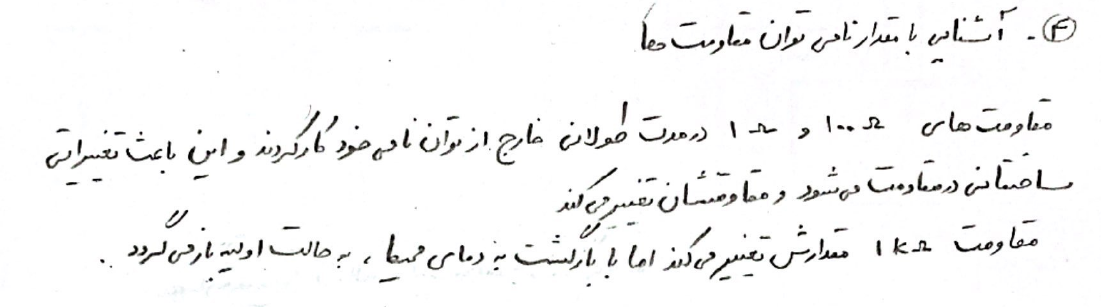
\includegraphics[width = \textwidth]{Q4/pish.png}}
    \caption{\textcolor{blue}{از پیش گزارش داریم}}
\end{figure}
از آزمایش واقعی:
مقادیر اندازه گیری شده در شروع آزمایش : $R_1 =989.6\Omega  , R_2=96.63\Omega , R_3=6.9 \Omega$
\subsection{مقاومت $1k\Omega$}
دو سر مقاومت را به ولتاژ 15 ولتی وصل میکنیم و سپس 
بعد از اینکه زمانی گذشت کمی داغ شده ولی طبق اینکه
در توان نامینال خود بوده بعد از اندازه گیری مقدار تغییر 
ناچیزی کرده و بعد از خنک شدن به مقدار قبلی خود باز میگردد\\
\subsection{مقاومت $100\Omega$}
این مقاومت را نیز به منبع 15 ولتی وصل میکنیم و در نتیجه مقاومت ما به شدت داغ میشود و بعد از مدتی
که اندازه میگیریم مقاومت به 96 اهم میرسد ولی در زمان کم کم ریکاوری میکند.\\
البته قابل توجه است که اگر مدت زمان بیشتری بذاریم این مقاومت ممکن است بسوزد و دیگر ریکاوری نکند.\\
\subsection{مقاومت $10\Omega$}
برای اطمینان مقاومت را به 6 ولت وصل میکنیم. ولی قابل توجه است که در این ولتاژ هم زمانی که
در حال اندازه گیری هستیم به طور ممد در حال کم شدن و شدیدا داغ شدن است مقاومت و مورد پیش بینی 
ساختار آن در حال تغییر است.\\
بعد از قطع کردن و حتی خنک شدن نیز روند نزولی تموم شده ولی مقاومت مقدار قابل توجهی تغییر کرده است
و اثری از ریکاوری نیست.\\
این مقاومت به طور کلی خراب شده است.\\

\pagebreak